%
% teil5.tex -- Das Napoleon-Dreieck
%
\section{Das Napoleon-Dreieck
\label{komplex:section:napoleon}}
\kopfrechts{Das Napoleon-Dreieck}
Mit den Werkzeugen aus Abschnitt~\ref{komplex:section:gleichseitig}
lässt sich nun das eigentliche Untersuchungsobjekt der Arbeit konstruieren.
Die folgenden Unterabschnitte beleuchten zunächst den historischen
Hintergrund, dann die geometrische Konstruktion,
ihre algebraische Übersetzung und schliesslich ein numerisches
Fallbeispiel.

%
% Historischer Hintergrund und Bedeutung
%
\subsection{Historischer Hintergrund und Bedeutung
\label{komplex:subsection:historisch}}
Der Satz von Napoleon trägt seinen Namen nach Napoleon Bonaparte,
\index{Napoleon Bonaparte}%
dem die Aussage zugeschrieben wird,
obwohl die historische Quellenlage nicht eindeutig ist.
Die erste belegte Veröffentlichung erfolgte 1825 in einer englischen
Zeitschrift.
Unabhängig von der Frage, wer den Satz tatsächlich entdeckte,
gilt er heute als ein klassisches Beispiel der elementaren Geometrie
und als eines der schönsten Anwendungsbeispiele für komplexe Zahlen
in der Geometrie der Ebene; vergleiche etwa~\cite{komplex:wells}
und~\cite{komplex:coxeter}.

Die praktische Anwendbarkeit des Satzes ist gering:
Im Bauwesen oder in der Vermessung spielt er keine Rolle.
Sein Wert liegt im intellektuellen Bereich.
Der Satz zeigt, dass aus einem völlig beliebigen Dreieck durch eine
einfache Konstruktion immer ein gleichseitiges Dreieck entsteht ---
ein erstaunliches Resultat, das Symmetrie aus Asymmetrie erzeugt.
Genau diese Eigenschaft macht ihn zu einem dankbaren Studienobjekt:
Er ist einfach genug, um vollständig durchgerechnet zu werden,
und überraschend genug, um der Mühe wert zu sein.

%
% Geometrische Konstruktion
%
\subsection{Geometrische Konstruktion
\label{komplex:subsection:konstruktion}}
Die Konstruktion verläuft in zwei Schritten,
die in Abbildung~\ref{komplex:figure:napoleon} dargestellt sind.
\begin{enumerate}
\item
Über jeder der drei Seiten eines beliebigen Dreiecks $ABC$ wird ein
gleichseitiges Dreieck nach aussen errichtet.
Damit entstehen drei zusätzliche Punkte, die mit $P_a$, $P_b$, $P_c$
bezeichnet werden.
Dabei ist $P_a$ der dritte Eckpunkt des über der Seite $BC$ liegenden
gleichseitigen Dreiecks (gegenüber von $A$),
$P_b$ der dritte Eckpunkt über $CA$ (gegenüber von $B$)
und $P_c$ der dritte Eckpunkt über $AB$ (gegenüber von $C$).
\item
Anschliessend werden die Schwerpunkte der drei aussen errichteten
gleichseitigen Dreiecke bestimmt.
Diese drei Schwerpunkte werden mit $O_a$, $O_b$, $O_c$ bezeichnet.
Der Satz von Napoleon besagt, dass das Dreieck $O_a O_b O_c$ gleichseitig
ist.
\end{enumerate}

%
% fig/napoleon.tex -- Napoleon-Dreieck am konkreten Beispiel
% A = 8 + 20i, B = 28 + 22i, C = 17 + 25i (gemaess Praesentation).
% Wir verschieben den Schwerpunkt in den Ursprung und skalieren mit 0.2,
% damit das Bild auf die Seite passt.
%
\begin{figure}
\centering
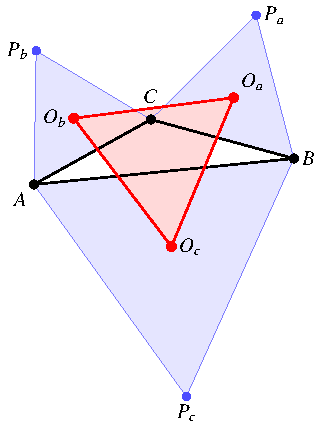
\includegraphics{papers/konstruktion/images/napoleon.pdf}
\caption{Konstruktion zum Satz von Napoleon am Beispiel
$A = 8 + 20i$, $B = 28 + 22i$, $C = 17 + 25i$.
Über jeder Seite des Ausgangsdreiecks $ABC$ (schwarz) wird ein
gleichseitiges Dreieck nach aussen errichtet (blau).
Die Schwerpunkte $O_a$, $O_b$, $O_c$ dieser drei aussen errichteten
Dreiecke bilden das Napoleon-Dreieck (rot), das stets gleichseitig ist.
\label{komplex:figure:napoleon}}
\end{figure}


Bemerkenswert ist, dass diese Aussage für jedes Ausgangsdreieck gilt ---
gleichseitige, gleich\-schenk\-lige, recht\-winklige oder völlig
unregelmässige.
Sie ist ferner stabil unter Translation, Rotation und Streckung des
Ausgangsdreiecks:
Verschiebt, dreht oder skaliert man $ABC$,
so verschieben, drehen und skalieren sich auch die drei Schwerpunkte mit,
und das Resultat bleibt gleichseitig.

%
% Algebraische Beschreibung mit komplexen Zahlen
%
\subsection{Algebraische Beschreibung mit komplexen Zahlen
\label{komplex:subsection:algebraisch-napoleon}}
Wir codieren das Aus\-gangs\-dreieck durch drei kom\-plexe Zahlen
$A, B, C$ und führen für die Ver\-bindungs\-strecken die Abkürzungen
\begin{equation}
z_{BA} = A - B ,
\qquad
z_{AC} = C - A ,
\qquad
z_{CB} = B - C
\label{komplex:eq:verbindungsstrecken}
\end{equation}
ein.
Mit dem Drehfaktor $d = \cos(60^\circ) + i \sin(60^\circ)$ und der
Drehformel \eqref{komplex:eq:dreieck} entstehen die drei aussen
errichteten Eckpunkte als
\begin{equation}
P_a = C + d \cdot z_{CB} ,
\qquad
P_b = A + d \cdot z_{AC} ,
\qquad
P_c = B + d \cdot z_{BA} .
\label{komplex:eq:p-punkte}
\end{equation}
Die Wahl des Drehsinns ist dabei so getroffen, dass die Spitzen für ein
positiv (gegen den Uhrzeigersinn) nummeriertes Ausgangsdreieck nach aussen
zeigen.

Die drei Schwerpunkte ergeben sich nach Formel
\index{Schwerpunkt}%
\eqref{komplex:eq:schwerpunkt} als arithmetisches Mittel der jeweiligen
drei Eckpunkte:
\begin{equation}
O_a
=
\frac{B + C + P_a}{3} ,
\qquad
O_b
=
\frac{A + C + P_b}{3} ,
\qquad
O_c
=
\frac{A + B + P_c}{3} .
\label{komplex:eq:schwerpunkte}
\end{equation}
Diese drei Ausdrücke sind das Werkzeug,
mit dem in Abschnitt~\ref{komplex:section:beweis} die Gleich\-seitig\-keit
des Schwer\-punkt\-dreiecks nachgewiesen wird.
\index{Schwerpunktdreieck}%

%
% Numerisches Fallbeispiel
%
\subsection{Numerisches Fallbeispiel
\label{komplex:subsection:fallbeispiel}}
Zur Verdeutlichung sei das Ausgangsdreieck mit
$A = 8 + 20i$, $B = 28 + 22i$, $C = 17 + 25i$ gewählt ---
ein bewusst unregelmässiges Dreieck.
Die Verbindungsstrecken lauten
\begin{equation}
z_{BA} = -20 - 2i ,
\qquad
z_{AC} = 9 + 5i ,
\qquad
z_{CB} = 11 - 3i .
\label{komplex:eq:beispiel-z}
\end{equation}
Mit $d = \tfrac{1}{2} + \tfrac{\!\sqrt{3}}{2} \, i$ liefert die Drehung der
Verbindungsstrecken um $60^\circ$
\begin{align}
z_{BA} \cdot d
&=
(-10 + \!\sqrt{3}) + (-1 - 10\!\sqrt{3}) \, i ,
\notag \\
z_{AC} \cdot d
&=
\frac{9 - 5\!\sqrt{3}}{2} + \frac{5 + 9\!\sqrt{3}}{2} \, i ,
\label{komplex:eq:beispiel-zd}
\\
z_{CB} \cdot d
&=
\frac{11 + 3\!\sqrt{3}}{2} + \frac{11\!\sqrt{3} - 3}{2} \, i .
\notag
\end{align}
Daraus ergeben sich die Eckpunkte der aussen errichteten Dreiecke
\begin{equation}
P_a \approx 25.10 + 33.03 \, i ,
\qquad
P_b \approx 8.17 + 30.29 \, i ,
\qquad
P_c \approx 19.73 + 3.68 \, i ,
\label{komplex:eq:beispiel-p}
\end{equation}
und die drei Schwerpunkte
\begin{equation}
O_a \approx 23.37 + 26.68 \, i ,
\qquad
O_b \approx 11.06 + 25.10 \, i ,
\qquad
O_c \approx 18.58 + 15.23 \, i .
\label{komplex:eq:beispiel-o}
\end{equation}
Eine kurze Rechnung bestätigt, dass die Abstände
$|O_a - O_b| = |O_b - O_c| = |O_c - O_a|$ alle gleich sind ---
das Dreieck $O_a O_b O_c$ ist tatsächlich gleichseitig,
eine numerische Bestätigung des allgemeinen Satzes,
dessen Beweis nun folgt.
